	\subsection{Skift adgangskode}
	Dette afsnit vil indeholde en gennem gang af design, grafisk bruger interface og implentering af Skift adgangskode activityen til android applikationen
	
	\subsubsection{Design}
	Skift adgangskode er designet efter samme fremgangsmåde som opret bruger. Det kan ses på figur \vref{fig:OpretBrugerSekvens}. Hvor input felterne bliver valideret, og udfra dette gives der feedback til brugeren om eventuelle fejl. 
	
	\subsubsection{Grafisk Bruger Interface}
	Layout for at skifte adgangskode på brugeren som er logget ind, kan ses på figur \vref{fig:Skift adgangskode på android applikationen}.	
	\begin{figure} [!ht]
		\begin{center}
			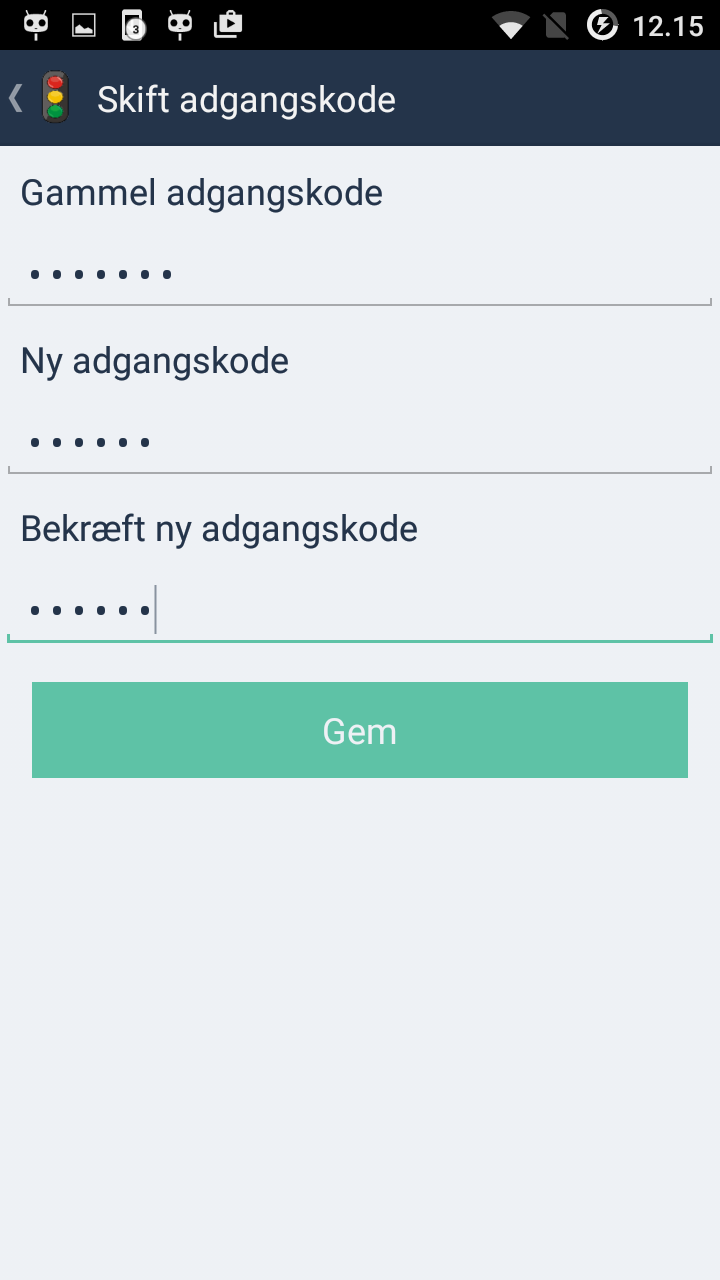
\includegraphics[height=10cm]{Android/Billeder/AndroidSkiftAdgangskode}
		\end{center}
		\caption{Skift adgangskode på android applikationen}
		\label{fig:Skift adgangskode på android applikationen}
	\end{figure}
	
	\subsubsection{Implementering}
	Når en brugen forsøger at skifte adgangskode, validerer presenteren at der er indtastet information, samt at den nye adgangskode passer overens med den beskræftede kode, inden informationen bliver sendt videre til modellen. Hvis et felt ikke er udfyldt giver presenteren besked til viewet om at en fejlbesked om dette, skal vises. Hvis alle de påkrævet felter er fyldt ud bliver et request sendt til API'et, gennem Modellen og DAL-laget.
	
	\pagebreak